\documentclass[a4paper]{article}
\renewcommand{\rmdefault}{ftm}
\usepackage[12pt]{extsizes}
\usepackage[utf8]{inputenc}
\usepackage[russian]{babel}
\usepackage{enumitem}
\usepackage{graphicx}
\setlist[enumerate]{itemsep=0mm}
\usepackage{setspace,amsmath}
\usepackage[left=25mm, top=15mm, right=10mm, bottom=25mm, nohead, footskip=10mm]{geometry}
\begin{document}
\begin{center}
\hfill \break
\large{\textbf{ФГБОУ ВО«Московский Политехнический университет»}}\\
\hfill \break
\hfill \break
\hfill \break
\hfill \break
\hfill \break
\hfill \break
\hfill \break
\large{Лабораторная работа№3}\\
\footnotesize{Линейные программы\\
Задание 1,2,3\hspace{3cm}Вариант№1\break\\
По дисциплине:\\
Основы Программирования
}
\end{center}
\hfill \break
\hfill \break
\hfill \break
\hfill \break
\hfill \break
\hfill \break
\hfill \break
\hfill \break
\hfill \break
\hfill \break
\normalsize{
\begin{tabular}{ccc}
\hspace{4cm}Выполнил & Шукуров Ф.Ф  & группа 181-362\\
\\
\hspace{4cm}Проверил & \underline{\hspace{3cm}}& Никишина И.Н
\end{tabular}
}
\hfill \break
\hfill \break
\hfill \break
\hfill \break
\hfill \break
\hfill \break
\hfill \break
\hfill \break
\hfill \break
\hfill \break
\hfill \break
\hfill \break
\hfill \break
\hfill \break
\hfill \break
\begin{center}\texttt{Москва 2018}\end{center}
\thispagestyle{empty}

\newpage
Лабораторная работа №3
\\
    \begin{lab3.1}
        \begin{center}\underline{\hspace{6cm}}\\
            Задание№1\\
        \end{center}
        Постановка задачи:\hspace{5mm} Вычислить и вывести на экран или в файл в виде таблицы значения функции, заданной графически \textsc{(см. лабораторная работа №2, задание 1)}, на интервале от X\small{нач}\normalsizeдо X\small{кон}\normalsize с шагом dx. Интревал и шаг задавать таким образом, чтобы поверить все веткви программы. Таблицу снабдить заголовком и  шапкой
    \begin{description}
        Описание программы:\\
        Программа была написана на алгоритмическом языке python v3.6, реализованна в среде os Linux, и состоит из блоков ввода, проверки информации и вывода результата. Использован импорт random для вывода <<Псведо случайного числа>>
    \end{description}
    \begin{algoritm}
        Описание Алгоритма:
        \small\begin{enumerate}
            \item Объевляем две переменные <<xBeg>>,<<xEnd>>,<<dx>>, присваиваем их к значению float
            \item <<xt>> будет ссылаться на данные <<xBeg>>.
            \item Выводим шапку программы
            \item Запускаем цикл \textsc{While} с уловием <<x $\leq$ xEnd>>
            \item Используя методы исключения (реализованным в python блок if $\to$ elif $\to$ else) находим <<xt>>
            \item Выводим информацию на экран
            \item Добовляем к <<xt>> шаг <<dx>>
            \item Как только <<xt>> становится $\leq$ xEnd, цикл While прекращается
        \end{enumerate}
    \begin{center}
        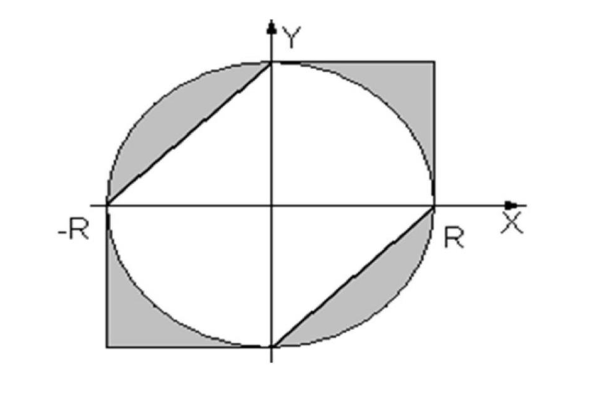
\includegraphics[width=100mm,scale=0.5]{for_lab_2_last.png}
    \end{center}
    \begin{comment}
        \footnotesize\textsc{{\texttt{Замечание: Цикл \textsc{While} может принимать значение \textsc{True} или \textsc{False}}}}
    \end{comment}
    \end{algoritm}\\
        \texttt{Листинг Программы:}
        \begin{verbatim}
# -*- coding: utf-8 -*-
from math import *
import random, math
xBeg = float(input("xBeg = "))
xEnd = float(input("xEnd = "))
dx = float(input("dx = "))
print("xBeg={0: 7.2f} xEnd={1: 7.2f}".format(xBeg,xEnd))
print("  dx={0:7.2f}".format(dx))
xt=xBeg
print("+--------+--------+")
print("I    X   I    Y   I")
print("+--------+--------+")
while xt<=xEnd:
    if xt <=-2.5: y = -6/7*xt-36/7
    elif -2.5<xt and xt<2: y = xt**3 + 1.5*xt**2-2.5*xt-3
    elif 2<=xt: y = -2*xt + 10
    print("I{0: 7.2f} I{1: 7.2f} I".format(xt,y))
    xt+=dx
            \end{verbatim}
    \begin{center}Результат работы программы:
        \begin{verbatim}
xBeg = 12
xEnd = 24
dx = 1
xBeg=  12.00 xEnd=  24.00
  dx=   1.00
+--------+--------+
I    X   I    Y   I
+--------+--------+
I  12.00 I -14.00 I
I  13.00 I -16.00 I
I  14.00 I -18.00 I
I  15.00 I -20.00 I
I  16.00 I -22.00 I
I  17.00 I -24.00 I
I  18.00 I -26.00 I
I  19.00 I -28.00 I
I  20.00 I -30.00 I
I  21.00 I -32.00 I
I  22.00 I -34.00 I
I  23.00 I -36.00 I
I  24.00 I -38.00 I
+--------+--------+

        \end{verbatim}
    \end{center}
    \end{lab3.1}
    \begin{lab3.2}
        \begin{center}
            \underline{\hspace{6cm}}\\
            Задание№2
        \end{center}\\

        \texttt{Постановка задачи:}\hspace{5mm}Для десяти выстрелов, координаты которых задаются генератором слуайных чисел, вывести текстовые сообщения о попаданни в мишень(см.лабораторная работа №2,задание 2)
    \begin{description}
        Описание программы:\\
        Программа была написана на алгоритмическом языке python v3.6, реализованна в среде os Linux, и состоит из блоков ввода, проверки информации и вывода результата. Использован импорт random для вывода <<Псведо случайного числа>>, а так же функции
        def \underline{name} (\underline{\hspace{1mm}}), аргумент global \underline{аргумент} позволяет ссылаться на аргументы из глобального пространства в локальное.
    \end{description}
    \begin{algoritm}
        Описание Алгоритма:
        \small\begin{enumerate}
        \item Создаем переменные <<t>>,<<f>> $\to$ присваиваем их к значению \textsc{int()}
        \item Используя input() в цикле for \underline{\hspace{1mm}} in range(\underline{\hspace{1cm}}), мы указываем количество выстрелов.
        \item Задавая <<RADUIS>>, <<x>>,<<y>> ~-- псевдо-случайное число используя ранеее импортированную функцию random.randrange(\underline{\hspace{2mm}})
        \item Используя блок исключений if $\to$ elif $\to$ else, мы исключаем попадание точек в опеределенную четверть оси координат, при значении if \underline{True} выполняется вызов функции <<two four()>> или <<one three()>>, в которых продолжаются дальнейшие вычисления
        \item В функциях проверяется принадлежность точки к заштрихованной части графика. В случае \texttt{истины}, переменной <<t>> прибавляется 1. В случае \texttt{не истины} к переменной <<f>> прибавляется 1.
        \item В случае нестандартных значений, которые не принадлежат графику, используется функция \texttt{error()}
        \end{enumerate}
    \begin{center}
        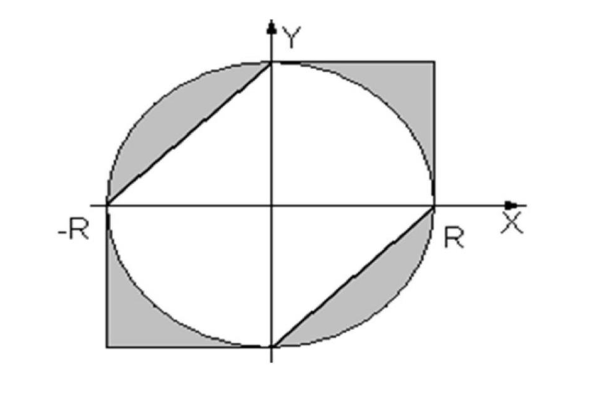
\includegraphics[width=100mm,scale=0.5]{for_lab_2_last.png}
    \end{center}
    \begin{comment}
        \footnotesize\textsc{{\texttt{Замечание: Цикл \textsc{While} может принимать значение \textsc{True} или \textsc{False}}}}
    \end{comment}
    \end{algoritm}\\

\normalsize\texttt{Листинг программы:}
\begin{verbatim}
def error():
    global f
    f+=1
    print('Мимо')
def true():
    global t
    t+=1
    print('Попал')
def two_four():
    if x>0 and y<0 and y<x-RADUIS:
        true()
    elif (x<0 and y>0) and y>x+RADUIS:
        true()
    else:
        error()
def one_three():
    if x<0 and y<0 and y<-x-RADUIS:
        true()
    elif x>0 and y>0 and y>-x-RADUIS:
        true()
    else:
        error()
t = int()
f = int()
for i in range(int(input("Введите количество выстрелов: \n"))):
    RADUIS = random.randrange(100)
    x = random.randrange(100)
    y = random.randrange(100)
    po_r = sqrt(x**2+y**2)  # point_radius
    if math.fabs(x)<=RADUIS and math.fabs(y)<=RADUIS:
        if po_r<=RADUIS:
            if (x<0 and y>0) or (y<0 and x>0): #первая и четвертая четверть
                two_four()
            else:
                error()
        elif po_r>=RADUIS:
            if (y>0 and x>0) or (x<0 and y<0):
                one_three()
            else:
                error()
        else:
            error()
    else:
        error()
print("Выстрелов попавших в цель: " + str(t))
print("Выстрелов не попавших в цель: " + str(f))
\end{verbatim}
\begin{center}Работа программы:\end{center}
\begin{verbatim}
Введите количество выстрелов:
10
Мимо
Мимо
Мимо
Мимо
Попал
Мимо
Мимо
Мимо
Мимо
Мимо
Выстрелов попавших в цель: 1
Выстрелов не попавших в цель: 9

\end{verbatim}
    \end{lab3.2}
    \begin{lab3.3}
        \begin{center}\underline{\hspace{6cm}}\\
            Задание№3\\
            Постановка задачи:\hspace{5mm}Вычислять и вывести на экран в виде таблицы значения функции $(1+x)^\frac{-1}{3}$ заданной рядом Тейлора $\to$\\
            \hspace{2cm}$1-\frac{1}{1\cdot2}(2\cdot3\cdot x-3\cdot4\cdot x^2+4\cdot5\cdot x^3-5\cdot6\cdot x^4+...)$\hspace{2cm}|x|\leq1\\
            на интервале от X\footnotesize{нач} до X\footnotesize{кон} с шагом dx с точностью $\epsilon$
        \end{center}
        \begin{description}
        Описание программы:\\
            Программа была написана на алгоритмическом языке python v3.6, реализованна в среде os Linux, и состоит из блоков ввода, проверки информации и вывода результата. Использован цикл <<While>>, а так же блоки проверки истинности.
        \end{description}
        Описание Алгоритма:
        \begin{algoritm}
        \small\begin{enumerate}
            \item Создаем бесконечный цикл в бесконечном цикле <<While \underline{True} $\to$ While \underline{True}>> для будущей проверки переменной xBeg, которую будет указывать пользователь.
            \item Если число введенной пользователем по модулю |xBeg| $\leq$ 1, выход из цикла
            \item Начинается проверка xEnd
            \item Если |xEnd| $\leq$ 1, выход из цикла
            \item Вывод шапки
            \item Создается переменная xt которая ссылается на xBeg (xt $\to$ xbeg)
            \item Запускаем цикл с уловием: xt $\leq$ xEnd, а так же в теле цикла создаем переменную result1, которая равна 0, а так же n которая равна 2.
            \item входим в цикл for, который будет выполнять действие количество раз, указанное пользователем.
            \item Проверяем счет цикла на чётность, методом получения остатка переменной i при делении на 2. При получении 0 $\to$ False, 1 $\to$ True. Следовательно, мы прибавляем либо отнимаем от result1 ответ формулы $n\cdot(n+1)\cdot xt^(^n^-^1^)$
            \item вывод 1-$\frac{result1}{2}$ на экран
            \item добавление к xt шаг dx
        \end{enumerate}
    \end{algoritm}\\
    \begin{verbatim}
while True:
    while True:
        xBeg = float(input("xBeg[-1:1]= "))
        if abs(xBeg)<=1:
            break
    xEnd = float(input("xEnd[-1:1] = "))
    if abs(xEnd)<=1:
        break
dx = float(input("dx = "))
print("xBeg={0: 7.2f} xEnd={1: 7.2f}".format(xBeg,xEnd))
print("dx={0:7.2f}".format(dx))
xt=xBeg
print("+---------+----------+")
print("I    X    I     Y    I")
print("+---------+----------+")
while xt<=xEnd:
    result_1 = 0
    n=2
    for i in range(int(input("Укажите точность расчетов:\t"))):
        if i%2: result_1-= (n*(n+1)*xt**(n-1))
        else:   result_1+= (n*(n+1)*xt**(n-1))
        n+=1
    print("I{0: 7.2f}  I {1: 7.2f}  I".format(xt, (1-result_1/2)))
    xt+=dx
    result_1 = 0
print("+---------+----------+")

    \end{verbatim}
\begin{center}
    Результат работы программы:
    \begin{verbatim}
xBeg[-1:1]= 0.01
xEnd[-1:1] = 1
dx = 0.1
xBeg=   0.01 xEnd=   1.00
dx=   0.10
+---------+----------+
I    X    I     Y    I
+---------+----------+
I   0.01  I    0.97  I
I   0.11  I    0.73  I
I   0.21  I    0.56  I
I   0.31  I    0.44  I
I   0.41  I    0.36  I
I   0.51  I    0.29  I
I   0.61  I    0.24  I
I   0.71  I    0.21  I
I   0.81  I    0.58  I
I   0.91  I   14.56  I
+---------+----------+

    \end{verbatim}
\end{center}
    \end{lab3.3}
\end{document}
